\documentclass[11pt]{article}

\usepackage[lmargin=0.75in, rmargin=1in, tmargin=1.25in, bmargin=1in]{geometry}
\usepackage[english]{babel}
\usepackage[utf8]{inputenc}

\usepackage{amsfonts}
\usepackage{amsmath}
\usepackage{bm}
\usepackage{booktabs}
\usepackage[labelsep=period]{caption}
\usepackage{enumitem}
\usepackage{fancyhdr}
\usepackage{graphicx}
\usepackage{lastpage}
\usepackage{listings}
\usepackage[svgnames]{xcolor}
\usepackage{float}
\usepackage{array}
\usepackage{subcaption}
\newcolumntype{P}[1]{>{\centering\arraybackslash}p{#1}}
\newcolumntype{M}[1]{>{\centering\arraybackslash}m{#1}}
\usepackage{scalerel}
\newcommand\Tau{\scalerel*{\tau}{T}}

% For formatting C++ code listings ---------------------------
\lstdefinestyle{customCpp}{
    language=C++,
    keywordstyle=\color{RoyalBlue},
    basicstyle=\footnotesize\ttfamily,
    commentstyle=\color{Green}\ttfamily,
    rulecolor=\color{black},
    numbers=left,
    numberstyle=\tiny\color{gray},
    stepnumber=1,
    numbersep=8pt,
    showstringspaces=false,
    breaklines=true,
    frame = tb,
    belowcaptionskip=5pt,
    belowskip=3em,
    gobble=10,
}

% For turning enumerated lists into Problem titles --------------
\renewcommand{\labelenumi}{\textbf{\arabic{enumi}.}}
\renewcommand{\labelenumii}{(\alph{enumii})}
\setlength\parindent{24pt}
\newcommand{\forceindent}{\leavevmode{\parindent=1em\indent}}

% Enumerated list indents:
% Problems:    [leftmargin=0.9in]
% Subproblems: [leftmargin=0.3in]


% Document Details ----------------------------------------------
\author{Eli Case}
\title{MECH 450 -- Homework 2}
\date{September, 14, 2023}
\makeatletter


% Setup headers -------------------------------------------------
\pagestyle{fancy}
\fancyhf{} % Clear the headers and footers
\lhead{\@author}
\chead{\@title}
\rhead{\@date}
\cfoot{Page \thepage\ of \pageref{LastPage}}
\setlength{\headheight}{15pt}
\setlength{\headsep}{20pt}

\fancypagestyle{plain}{
	\fancyhf{}
	\setlength{\headheight}{15pt}
	\setlength{\headsep}{0pt}
	\renewcommand{\headrulewidth}{0pt}
	\cfoot{\vspace{2mm}Page \thepage\ of \pageref{LastPage}}
}

\begin{document}
\flushleft
\thispagestyle{plain}

From: \@author

Date: \@date

Subject: \@title

\makeatother
\medskip
\hrule
\medskip

\begin{enumerate}[leftmargin=0.3in]

   \item % Problem 1
   \begin{enumerate}
    We would like to show that $\Tau$ and regular matrix multiplication form a group. It is also known that rotation matrices in the set $\mathit{SO}(2)$ with matrix multiplication form a group and that translation vectors in the set $\mathbb{R}^2$ with vector addition form a group. \break

    We can first demonstrate closure of $\Tau$ with matrix multiplication. Consider $\mathit{T}_1, \mathit{T}_2 \in \Tau$. 
       \begin{align*}
           \mathit{T}_1 \mathit{T}_2 &= \begin{bmatrix}
               \mathit{R}_1 & \mathit{p}_1 \\
               0 & 1
               \end{bmatrix} \begin{bmatrix}
               \mathit{R}_2 & \mathit{p}_2 \\
               0 & 1
           \end{bmatrix} \\
           &= \begin{bmatrix}
              \mathit{R}_1 \mathit{R}_2 & \mathit{R}_1 \mathit{p}_2 + \mathit{p}_1 \\
              0 & 1
          \end{bmatrix}
       \end{align*}

       Now, since $\mathit{SO}(2)$ with matrix multiplication forms a group and $\mathit{R}_1, \mathit{R}_2 \in \mathit{SO}(2)$, we have that $\mathit{R}_1 \mathit{R}_2 \in \mathit{SO}(2)$. Additionally, we have that $\mathit{p}_2 \in \mathbb{R}^2$ and that $\mathit{R}_2 \mathit{p}_1 \in \mathbb{R}^2$. Thus, since $\mathbb{R}^2$ and vector addition forms a group, $\mathit{R}_2 \mathit{p}_1 + \mathit{p}_2 \in \mathbb{R}^2$. As a result, we have that the elements of $\mathit{T}_1 \mathit{T}_2$ have closure, implying that $\mathit{T}_1 \mathit{T}_2 \in \Tau$ and thus the closure of $\Tau$ with matrix multiplication. \break 

       Next, we demonstrate the associativity of $\Tau$ with matrix multiplication. Consider $\mathit{T}_1, \mathit{T}_2, \mathit{T}_3 \in \Tau$.
       \begin{align*}
           ( \mathit{T}_1 \mathit{T}_2 ) \mathit{T}_3 &= \bigg( \begin{bmatrix}
              \mathit{R}_1 & \mathit{p}_1 \\
              0 & 1
              \end{bmatrix} \begin{bmatrix}
              \mathit{R}_2 & \mathit{p}_2 \\
              0 & 1
          \end{bmatrix} \bigg) \begin{bmatrix}
              \mathit{R}_3 & \mathit{p}_3 \\
              0 & 1
            \end{bmatrix} \\
              &= \begin{bmatrix}
                  \mathit{R}_1 \mathit{R}_2 & \mathit{R}_1 \mathit{p}_2 + \mathit{p}_1 \\
                  0 & 1
                  \end{bmatrix} \begin{bmatrix}
              \mathit{R}_3 & \mathit{p}_3 \\
              0 & 1
            \end{bmatrix} \\
              &= \begin{bmatrix}
                  \mathit{R}_1 \mathit{R}_2 \mathit{R}_3 & \mathit{R}_1 \mathit{R}_2 \mathit{p}_3 + \mathit{R}_1 \mathit{p}_2 + \mathit{p}_1 \\
                  0 & 1
              \end{bmatrix} \\
           \mathit{T}_1 ( \mathit{T}_2 \mathit{T}_3 ) &= \begin{bmatrix}
              \mathit{R}_1 & \mathit{p}_1 \\
              0 & 1
              \end{bmatrix} \bigg( \begin{bmatrix}
              \mathit{R}_2 & \mathit{p}_2 \\
              0 & 1
          \end{bmatrix} \begin{bmatrix}
              \mathit{R}_3 & \mathit{p}_3 \\
              0 & 1
            \end{bmatrix} \bigg) \\
            &= \begin{bmatrix}
              \mathit{R}_1 & \mathit{p}_1 \\
              0 & 1
              \end{bmatrix} \begin{bmatrix}
                \mathit{R}_2 \mathit{R}_3 & \mathit{R}_2 \mathit{p}_3 + \mathit{p}_2 \\
                0 & 1
              \end{bmatrix} \\
            &= \begin{bmatrix}
                \mathit{R}_1 \mathit{R}_2 \mathit{R}_3 & \mathit{R}_1 \mathit{R}_2 \mathit{p}_3 + \mathit{R}_1 \mathit{p}_2 + \mathit{p}_1\\
                0 & 1
            \end{bmatrix} \\
            &= (\mathit{T}_1 \mathit{T}_2 ) \mathit{T}_3
       \end{align*}
Thus, we have that $(\mathit{T}_1 \mathit{T}_2) \mathit{T}_3  = \mathit{T}_1 (\mathit{T}_2 \mathit{T}_3)$ and that $\Tau$ with matrix multiplication is associative. \break

Now, the identity of $\Tau$ with matrix multiplication will be shown. Let $\mathit{I}$ be the identity matrix as shown below.
   \begin{equation*}
       \mathit{I} = \begin{bmatrix}
    1 & 0 & 0 \\
    0 & 1 & 0 \\
    0 & 0 & 1
    \end{bmatrix}
   \end{equation*}
   $\mathit{I} \in \Tau$ since it can be formed with the following choices for a rotation matrix, $\mathit{R}$, and translation vector $\mathit{p}$. 
   \begin{align*}
       \mathit{R} &= \begin{bmatrix}
        1 & 0 \\
        0 & 1
    \end{bmatrix} \\
       \mathit{p} &= \begin{bmatrix}
           0 \\
           0
       \end{bmatrix}
   \end{align*}
   Denote the submatrix given by the above choice of $\mathit{R}$ as $\tilde{\mathit{I}}$ and the subvector given by the above choice of $\mathit{p}$ as $\mathit{0}$. Then, we write $\mathit{I}$ as follows.
   \begin{equation*}
       \mathit{I} = \begin{bmatrix}
               \tilde{\mathit{I}} & \mathit{0} \\
               0 & 1
       \end{bmatrix}
   \end{equation*}
   Now consider $\mathit{T} \in \Tau$.
   \begin{align*}
       \mathit{I} \mathit{T} &= \begin{bmatrix}
               \tilde{\mathit{I}} & \mathit{0} \\
               0 & 1
               \end{bmatrix} \begin{bmatrix}
               \mathit{R} & \mathit{p} \\
               0 & 1
           \end{bmatrix} \\ 
            &= \begin{bmatrix}
                \tilde{\mathit{I}} \mathit{R} & \mathit{p} \\
                0 & 1
            \end{bmatrix} \\
            &= \begin{bmatrix}
                \mathit{R} & \mathit{p} \\
                0 & 1
            \end{bmatrix} \\
            &= \mathit{T} \\
           \mathit{T} \mathit{I} &= \begin{bmatrix}
               \mathit{R} & \mathit{p} \\
               0 & 1
               \end{bmatrix} \begin{bmatrix} 
               \tilde{\mathit{I}} & \mathit{0} \\
               0 & 1
           \end{bmatrix} \\
            &= \begin{bmatrix}
                \mathit{R} \tilde{\mathit{I}} & \mathit{p} \\
                0 & 1
            \end{bmatrix} \\
            &= \begin{bmatrix}
                \mathit{R} & \mathit{p} \\
                0 & 1
            \end{bmatrix} \\
            &= \mathit{T}
   \end{align*}
   Thus, we have $\mathit{I} \mathit{T} = \mathit{T} \mathit{I} = \mathit{T}$ and the identity property for $\Tau$ with matrix multiplication. \break

   Lastly, the inverse property of $\Tau$ with matrix multiplication will be proved. Consider $\mathit{D} \in \Tau$ as defined below.
   \begin{align*}
       \mathit{D} &= \begin{bmatrix}
           \mathit{R}^{-1} & -\mathit{R}^{-1} p \\
          0 & 1
       \end{bmatrix} \\
       &= \begin{bmatrix}
           \mathit{R}^T & -\mathit{R}^T p \\
          0 & 1
       \end{bmatrix} ,
   \end{align*}
   where $\mathit{R}^{-1} = \mathit{R}^T \in \mathit{SO}(2)$ is the transpose of the orthogonal rotation matrix, $\mathit{R} \in \mathit{SO}(2)$. Now, we consider $\mathit{T} \in \Tau$.
   \begin{align*}
       \mathit{D} \mathit{T} &= \begin{bmatrix}
           \mathit{R}^T & -\mathit{R}^T p \\
           0 & 1
           \end{bmatrix} \begin{bmatrix}
           R & p \\
           0 & 1
       \end{bmatrix} \\
       &= \begin{bmatrix} 
           \mathit{R}^T \mathit{R} & \mathit{R}^T \mathit{p} - \mathit{R}^T \mathit{p} \\
           0 & 1
       \end{bmatrix} \\
       &= \begin{bmatrix}
           \tilde{\mathit{I}} & \mathit{0} \\
           0 & 1
       \end{bmatrix} \\
       &= \mathit{I} \\
           \mathit{T} \mathit{D} &= \begin{bmatrix} 
           R & p \\
           0 & 1 
           \end{bmatrix} \begin{bmatrix}
           \mathit{R}^T & -\mathit{R}^T p \\
           0 & 1
           \end{bmatrix} \\
           &= \begin{bmatrix}
               \mathit{R} \mathit{R}^T & - \mathit{R} \mathit{R}^T \mathit{p} + \mathit{p}\\
               0 & 1
           \end{bmatrix} \\
           &= \begin{bmatrix}
               \tilde{\mathit{I}} & - \tilde{\mathit{I}} \mathit{p} + \mathit{p} \\
               0 & 1
           \end{bmatrix} \\
           &= \begin{bmatrix}
               \tilde{\mathit{I}} & -\mathit{p} + \mathit{p} \\
               0 & 1
           \end{bmatrix} \\
           &= \begin{bmatrix}
               \tilde{\mathit{I}} & \mathit{0} \\
               0 & 1
           \end{bmatrix} \\
           &= \mathit{I}
   \end{align*}
   Thus, we have that $\mathit{D} = \mathit{T}^{-1}$ and that the identity property for $\Tau$ with matrix multiplication is satisfied.

   Since $\Tau$ with matrix multiplication satisfies closure, associativity, identity, and inverse, we conclude that it forms a group. $\square$

   \end{enumerate} % End of Problem 1 subpoints
   
   \item % Problem 2
   \begin{enumerate}
       \item We are given the unit quaternion $\mathit{q}_1 = \frac{\sqrt{2}}{2} + 0i + \frac{\sqrt{2}}{2}j + 0k$. Using the provided tool, we obtain the Euler Angle ZYX as $(\alpha, \beta, \gamma) = (0 ^\circ, 90 ^\circ, 0^\circ)$. We can recover the world's reference frame with the rotation given by the Euler angles ZYX $(\alpha, \beta, \gamma) = (0 ^\circ, -90 ^\circ, 0 ^\circ)$. Below in Figure \ref{fig:1}, the world's reference frame with respect to the robot is shown.

       \begin{figure}[H]
           \centering
           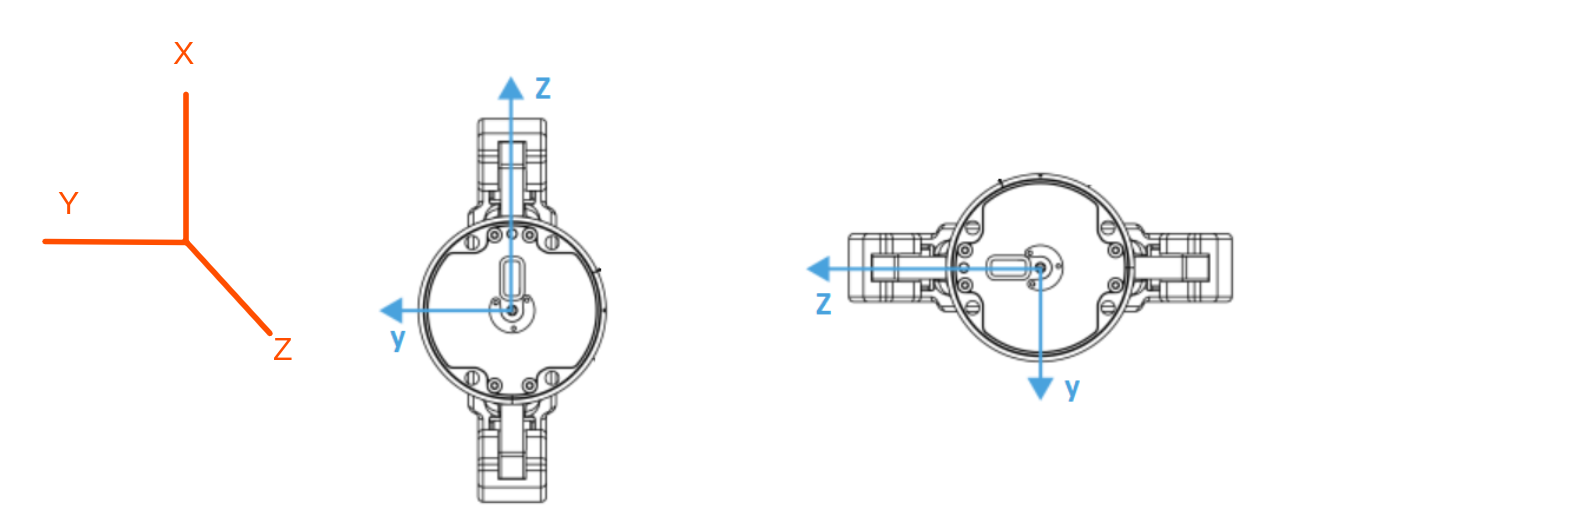
\includegraphics[width=16cm]{figures/Problem2.png}
               \caption{World Reference Frame}
               \label{fig:1}
           \end{figure}

       \item One can deduce that the Euler angles ZYX corresponding to the orientation shown in Figure 1b are $(\alpha, \beta, \gamma) = (0 ^\circ, 90 ^\circ, -90 ^\circ)$. These angles are found by examining Figure \ref{fig:1} provided in the answer in the previous part. We have a sequence of two rotations, the first being a $90 ^\circ$ rotation counter-clockwise about the $y-axis$ and the second being a $90 ^\circ$ clockwise rotation about the x-axis. Using this Euler Angle ZYX, we obtain the equivalent quaternion, $\mathit{q}_2$, as $\mathit{q}_2 = \frac{1}{2} - \frac{1}{2}i + \frac{1}{2}j + \frac{1}{2}k$. 

   \end{enumerate} % End of Problem 2 subpoints

\item %Problem 3 

    \begin{enumerate}
        \item For the left manipulator, there are $2$ DOF. Thus, the dimension of the manipulator's configuration space is $2$. We can parametrize each prismatic joint as $x_i \in \mathbb{R}$, $i = 0,1$, making the topology of the configuration space, $C = \mathbb{R} \times \mathbb{R} = \mathbb{R}^2$. 

        \item For the middle manipulator, there are $3$ DOF. Thus, the dimension of the manipulator's configuration space is $3$. We can again parametrize the prismatic joint as $x_i \in \mathbb{R}$ , $i = 0$. We can then parameterize each revolute joint as $u_i = \text{cos}(\theta) , r_i = \text{sin}(\theta)$, where $u_i^2 + r_i^2 = 1$, $i = 1, 2$. This parametrization results in a configuration space topology of $C = \mathbb{R} \times S^1 \times S^1 = \mathbb{R} \times T$.

\item For the right manipulator, there are $7$ DOF. Thus, the dimension of the manipulator's configuration space is $7$. We can parametrize each prismatic joint as $u_i = \text{cos}(\theta) , r_i = \text{sin}(\theta)$, where $u_i^2 + r_i^2 = 1$, $i = 1, ..., 7$. This parametrization results in a configuration space topology of $C = (S^1)^7$. 

    \end{enumerate}

\item %Problem 4 

    \begin{enumerate}
        \item For this manipulator, 4 DOF are identified: $x_1, y_1, \theta_1, \theta_2$. Thus, we have a configuration space dimension of $4$. We can parametrize the configuration space with $x_1 \in \mathbb{R}, y_2 \in \mathbb{R}$ and $u_i = \text{cos}(\theta_i), r_i = \text{cos}(\theta_i)$, with $u_i^2 + r_i^2 = 1$ for $i = 1, 2$. Thus, the topology of the configuration space will be $C = \mathbb{R} \times \mathbb{R} \times S^1 \times S^1 = \mathbb{R}^2 \times T$. 

        \item We can construct $\mathit{v}_3$ as shown below. 
            \begin{equation*}
                \mathit{v}_3 = \begin{bmatrix}
                   \mathit{l}_3 \\
                   0 \\ 
                   1
               \end{bmatrix}
            \end{equation*}

        \item We can compute $\mathit{v}_1$ as shown below.
            \begin{align*}
                \mathit{v}_1 = \begin{bmatrix}
                    \mathit{l}_1 + \mathit{l}_2 \text{cos}(\theta_2) + \mathit{l}_3 \text{cos}(\theta_2 + \theta_3) \\
                    \mathit{l}_2 \text{sin}(\theta_2) + \mathit{l}_3 \text{sin}(\theta_2 + \theta_3)\\
                    1
                \end{bmatrix}
            \end{align*}

        \item We can construct $\mathit{T}_2$ as follows.
            \begin{align*}
               \mathit{T}_2 = \begin{bmatrix}
                   \text{cos}(\theta_2) & -\text{sin}(\theta_2) & \mathit{l}_1 \\
                   \text{sin}(\theta_2) & \text{cos}(\theta_2) & 0 \\
                   0 & 0 & 1
               \end{bmatrix}
            \end{align*}
            
            Similarly, $\mathit{T}_3$ is given below.
            \begin{align*}
               \mathit{T}_3 = \begin{bmatrix}
                   \text{cos}(\theta_3) & -\text{sin}(\theta_3) & \mathit{l}_2 \\
                   \text{sin}(\theta_3) & \text{cos}(\theta_3) & 0 \\
                   0 & 0 & 1
               \end{bmatrix}
            \end{align*}

            Computing $\mathit{T}_2 \mathit{T}_3$, we have,
            \begin{align*}
                \mathit{T}_2 \mathit{T}_3 &= \begin{bmatrix}
                   \text{cos}(\theta_2) & -\text{sin}(\theta_2) & \mathit{l}_1 \\
                   \text{sin}(\theta_2) & \text{cos}(\theta_2) & 0 \\
                   0 & 0 & 1
                   \end{bmatrix} \begin{bmatrix}
                   \text{cos}(\theta_3) & -\text{sin}(\theta_3) & \mathit{l}_2 \\
                   \text{sin}(\theta_3) & \text{cos}(\theta_3) & 0 \\
                   0 & 0 & 1
               \end{bmatrix} \\
                  &= \begin{bmatrix}
                      c_{\theta_2} c_{\theta_3} - s_{\theta_2} s_{\theta_3} & -c_{\theta_2} s_{\theta_3} - s_{\theta_2} c_{\theta_3} & c_{\theta_2} \mathit{l}_2 + \mathit{l}_1 \\
                      s_{\theta_2} c_{\theta_3} + c_{\theta_2} s_{\theta_3} & -s_{\theta_2} s_{\theta_3} + c_{\theta_2} c_{\theta_3} & s_{\theta_2} \mathit{l}_2 \\
                      0 & 0 & 1
                  \end{bmatrix} \\
                  &= \begin{bmatrix}
                      \text{cos}(\theta_2 + \theta_3) & -\text{sin}(\theta_2 + \theta_3) & \text{cos}(\theta_2)\mathit{l}_2 + \mathit{l}_1 \\
                      \text{sin}(\theta_2 + \theta_3) & \text{cos}(\theta_2 + \theta_3) & \text{sin}(\theta_2) \mathit{l}_2 \\
                      0 & 0 & 1
                  \end{bmatrix}
            \end{align*}

        \item Computing, $\mathit{T}_2 \mathit{T}_3 \mathit{v}_3$, we have,
            \begin{align*}
                \mathit{T}_2 \mathit{T}_3 \mathit{v}_3 &= \begin{bmatrix}
                      \text{cos}(\theta_2 + \theta_3) & -\text{sin}(\theta_2 + \theta_3) & \text{cos}(\theta_2)\mathit{l}_2 + \mathit{l}_1 \\
                      \text{sin}(\theta_2 + \theta_3) & \text{cos}(\theta_2 + \theta_3) & \text{sin}(\theta_2) \mathit{l}_2 \\
                      0 & 0 & 1
                  \end{bmatrix}
                  \begin{bmatrix}
                      \mathit{v}_3 \\
                      0 \\
                      1
                  \end{bmatrix} \\
                  &= \begin{bmatrix}
                     \text{cos}(\theta_2 + \theta_3) \mathit{v}_3 + \text{cos}(\theta_2) \mathit{l}_2 + \mathit{l}_1 \\
                     \text{sin}(\theta_2 + \theta_3) \mathit{v}_3 + \text{sin}(\theta_2) \mathit{l}_2 \\
                     1
                  \end{bmatrix} \\
                  &= \mathit{v}_1
            \end{align*}

                As a result, we have that $\mathit{v}_1 = \mathit{T}_2 \mathit{T}_3 \mathit{v}_3$. $\square$ 

    \end{enumerate}

\item 

    \begin{enumerate}
        Denote the convex obstacle as $C_{obs}$, the workspace obstacle as $O$, and the convex robot as $A$. Consider $y_1, y_2 \in C_{obs}$. If $C_{obs}$ is a convex set, then $\forall y_1, y_2 \in C_{obs}, \forall \lambda \in [0,1]$
        \begin{equation*}
            \lambda y_2 + (1 - \lambda)y_1 \in C_{obs}
        \end{equation*}
        Now we know that $O, A$ are convex sets. Consider $o_1, o_2 \in O$ and $a_1, a_2 \in A$. We have the following.
        \begin{align*}
            \lambda o_2 + (1 - \lambda)o_1 \in O \\
            \lambda a_2 + (1 - \lambda)a_1 \in A
        \end{align*}
        We also know that the configuration space obstacle, $C_{obs}$ corresponding to workspace obstacle $O$ and robot $A$ can be presented with a Minkowski difference as follows.
        \begin{equation*}
            C_{obs} = O \ominus A = \{o - a | o \in O, a \in A\}
        \end{equation*}
        Now, consider again $y_1, y_2 \in C_{obs}$ We can write $y_1 = o_1 - a_1$ and $y_2 = o_2 - a_2$ for $o_1, o_2 \in O$ and $a_1, a_2 \in A$. Rearranging the definition for $O$ and $A$ being convex sets gives the following. 
        \begin{align*}
            \lambda o_2 + (1 - \lambda)o_1 - (\lambda a_2 + (1- \lambda) a_1)\in O \ominus A \\
            \lambda (o_2 - a_2) + (1 - \lambda) (o_1 - a_1) \in O \ominus A \\
            \lambda y_2 + (1 - \lambda) y_1 \in C_{obs} ,
        \end{align*}
        which is the definition of $C_{obs}$ being a convex set. Thus, $C_{obs}$ is a convex set. $\square$
    \end{enumerate}

\item 

    \begin{enumerate}
        Each polyhedral body can rotate and translate with respect to each other. Additionally, since they are treated as one composite robot, the composite robot is also collectively free to translate and rotate in space. We know for one rigid body in 3D space, there are 6 DoF, giving the configuration space a dimension of 6. SInce we have 6 bodies to consider in this scenario, we have 36 DoF, a subsequently, a configuration space with dimension 36. Additionally, the topology of a rigid body in 3D space is $SE(3)$, meaning the toplogy of the composite robot will be $SE(3)^6$.
    \end{enumerate}

\end{enumerate}

\end{document}
